\subsection{Description/additional circuitry}
Describe the type of the torque encoder(s) used, provide tables with main operation parameters, and describe additional circuitry used to check or manipulate the signal going to the motor controller. Describe how the system reacts if an implausibility or error (e.g. short circuit or open circuit or equivalent) is detected.

\begin{table}[H]
	\centering
	\caption{Torque encoder data}
	\begin{tabularx}{\textwidth}{|X|X|}
		\hline
		Torque encoder manufacturer: &  \\[\TableSize]\hline
		Torque encoder type: &  \\[\TableSize]\hline
		Torque encoder principle: &  \\[\TableSize]\hline
		Total number of Torque Encoder Sensors: &  \\[\TableSize]\hline
		Supply voltage: &  \\[\TableSize]\hline
		Maximum supply current: &  \\[\TableSize]\hline
		Operating temperature: &  \\[\TableSize]\hline
		Used output: &  \\[\TableSize]\hline
	\end{tabularx}%
	\label{tab:encoder-general}%
\end{table}%

\subsection{Torque Encoder Plausability Check}
Describe additional circuitry used to check or manipulate the signal going to the motor controller. Describe how failures (e.g. Implausibility, short circuit or open circuit or equivalent) are detected and how the system reacts if an implausibility or errors is detected.

\subsection{Wiring}
Describe the wiring, show schematics, show data regarding the cables and connectors used.

\subsubsection{Position in car/mechanical fastening/mechanical connection}
%Provide CAD-renderings showing all relevant parts and discuss the mechanical connection of the sensors to the pedal assembly. Mark the parts in the rendering, if necessary.

\begin{figure}[H]
	\centering
	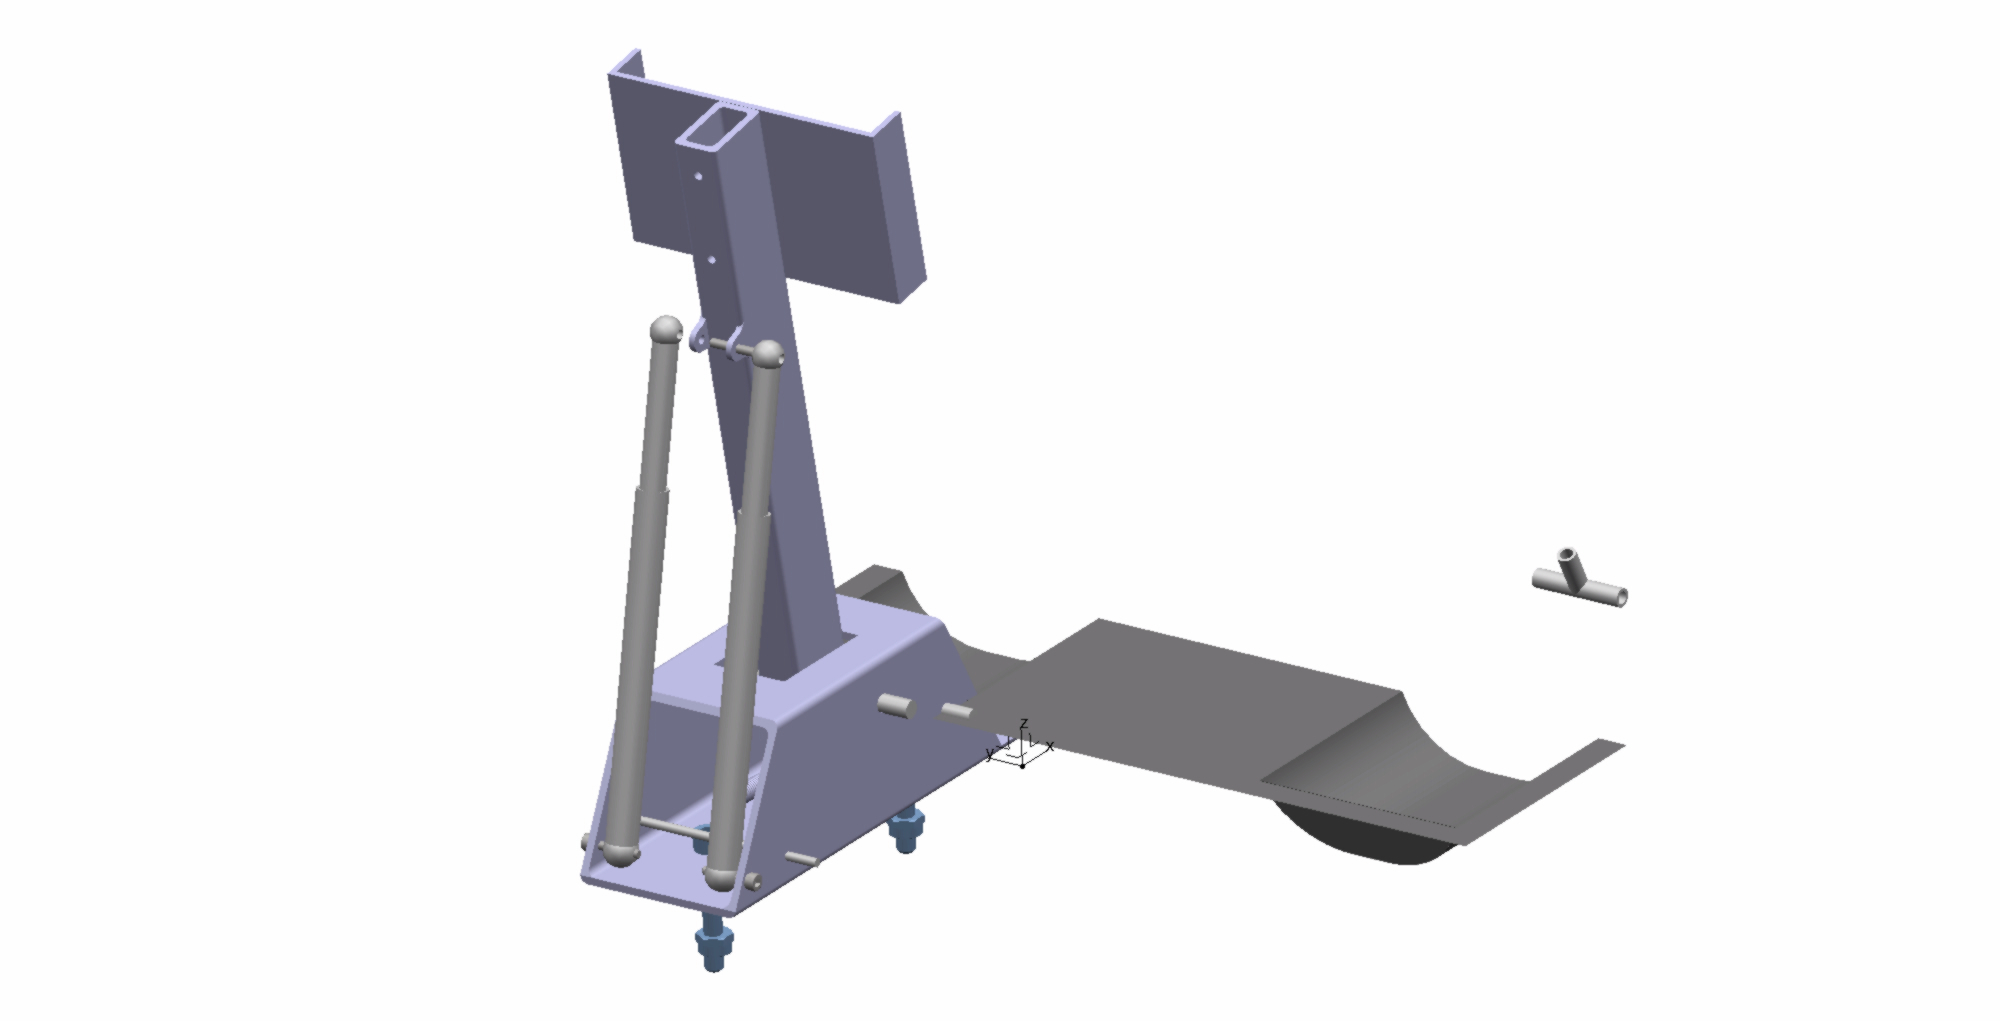
\includegraphics[width=.5\textwidth]{./img/ACC-pedal-pos.jpg}
	\caption{Accelerator pedal position.}
	\label{fig:ACC-position}
\end{figure}

\begin{figure}[H]
	\centering
	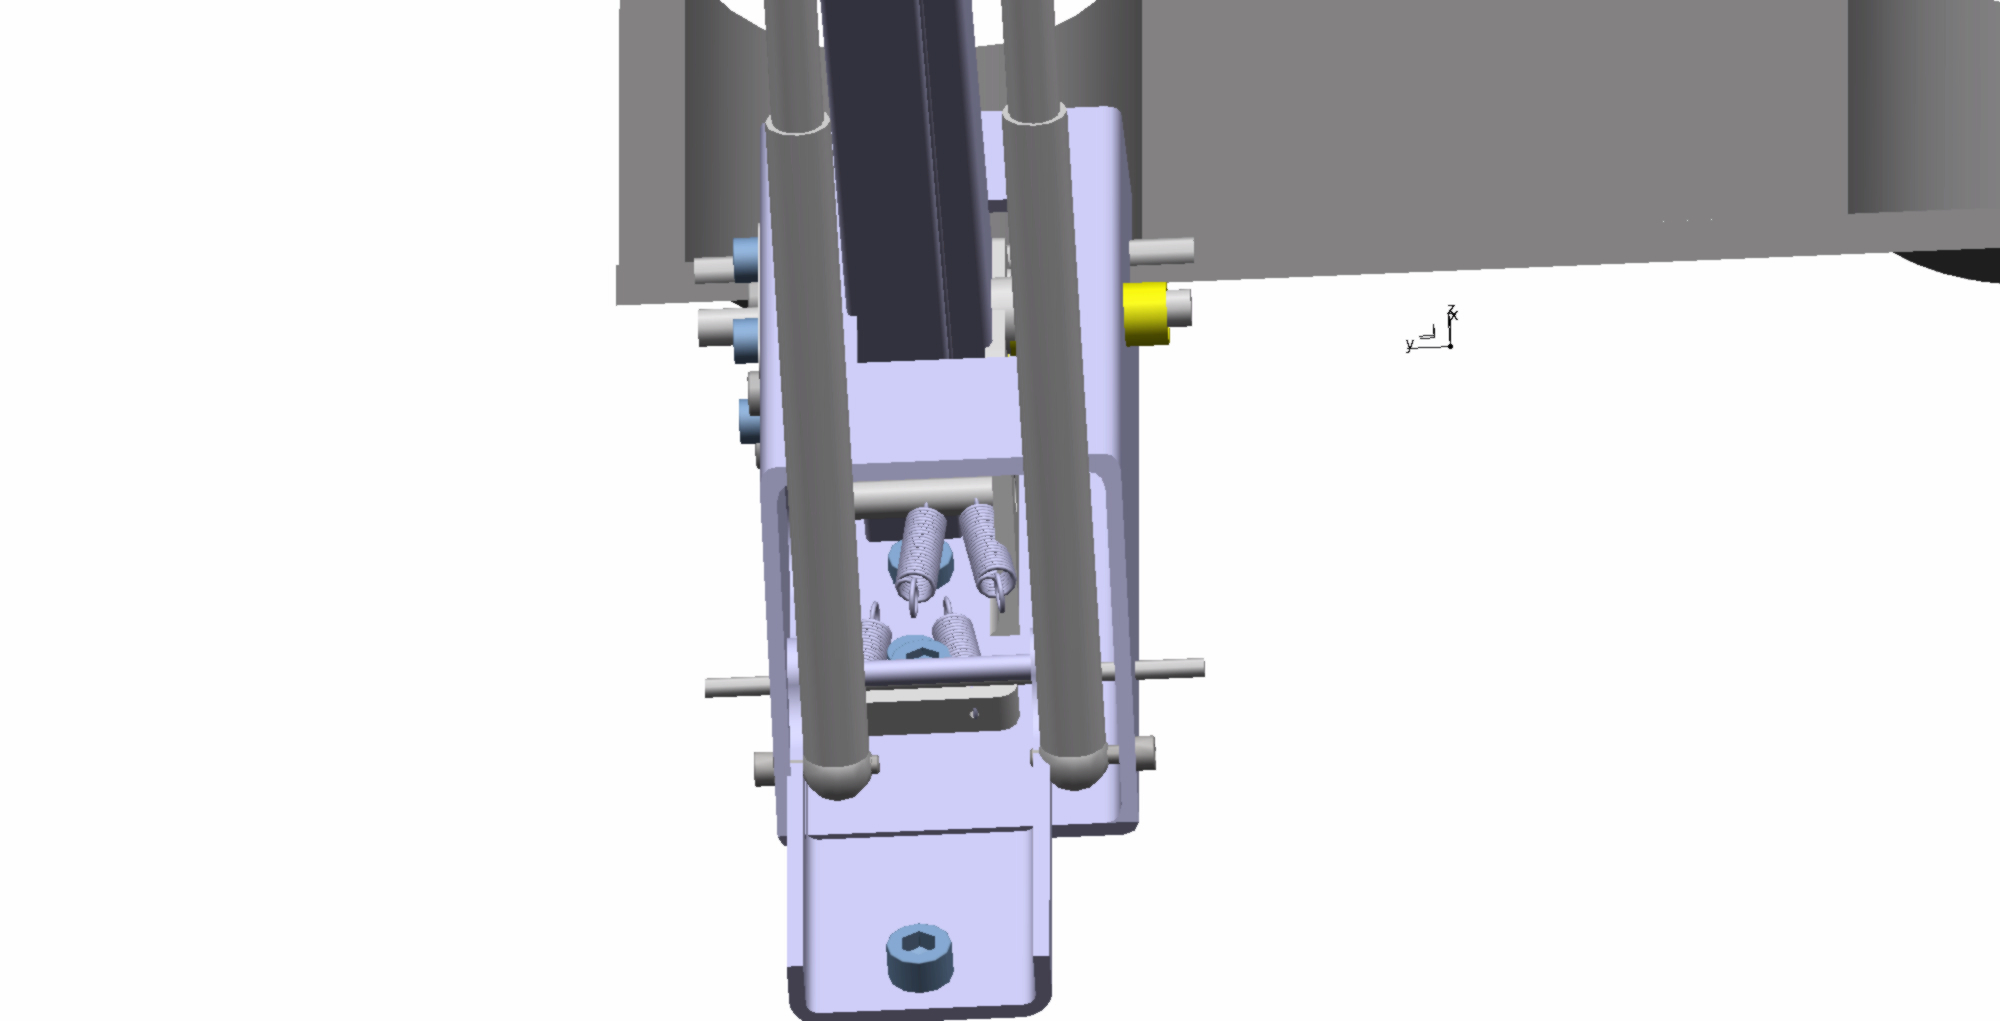
\includegraphics[width=.5\textwidth]{./img/ACC-pedal-pos2.jpg}
	\caption{Accelerator pedal position.}
	\label{fig:ACC-position2}
\end{figure}

